% !Mode:: "TeX:UTF-8"

\chapter{中断处理模块设计与实现}[interrupt]
\label{chapter:interrupt}

\section{模块概述}

\ref{sec:interrupt} 节中介绍过,RISC-V支持两种方式的中断处理,分别是Direct模式与Vectored模式。采用Direct模式时,当任意中断发生后,都会跳转到stvec中的BASE地址处;若是采用Vectored模式,则类似于Linux内核中使用的中断向量表,需要首先进行向量表的填充,不利于统一处理或忽略一些中断,且填表过程比较繁琐,所以Moonix中采用Direct模式来对中断进行统一处理。在中断处理函数中就可以很方便地根据中断类型来对不同的类型调用不同的处理函数分流处理流程。

在跳转进入中断处理函数之前,需要保存当前线程的CPU状态,并在退出之前恢复,以保证整个中断处理过程对线程来说是透明的。Moonix将CPU中所有的通用寄存器都保存在线程的内核栈上,并在中断函数处理结束之后将寄存器的值从内核栈上恢复到CPU,随后再跳转回原线程被中断打断的位置继续执行。

在Moonix中,中断处理需要处理以下三种最重要的中断:时钟中断、用户态(U-Mode)环境调用和外部串口中断。时钟中断主要用于线程调度,在每次时钟中断发生时,线程调度模块都会检查当前线程的时间片,来决定是否要继续执行,更具体内容将在第 \ref{chapter:thread} 章展开说明。用户态环境调用类似于Linux中的系统调用,用于U-Mode下进程向S-Mode下操作系统请求系统功能,如输入输出、文件读写等。外部串口中断主要用于实现用户输入,因为在QEMU中,键盘被实现为一个串口设备。用户输入是一个异步事件,不可预知,为了避免需要读取键盘的线程陷入无意义的忙循环等待中,Moonix使用条件变量来实现条件等待-恢复机制,条件变量与标准输入的实现细节将在 \ref{sec:condition} 节做更深入的讨论。

\section{中断上下文的保存与恢复}

\subsection{定义中断上下文}

对于一个程序来说,某一时刻寄存器的数据和栈中的数据可以唯一确定这个程序的运行状态,由于Moonix中程序栈使用内存实现,栈顶地址保存在CPU中的sp寄存器内。因此,保存一个程序的运行状态,只需要保存这个时刻CPU中所有的通用寄存器即可。Moonix中将保存程序运行状态的数据结构成为程序上下文。

对于被中断打断的程序来说,中断处理程序应当是透明的。流程从中断处理程序恢复到原先的程序时,应当继续执行被打断的流程,并且所有的中间变量都不应当被修改,否则可能导致原先的程序发生错误。

因此,在处理中断前,Moonix需要保存所有可能被修改的寄存器,并在中断处理完成后恢复。这些包括:所有的通用寄存器,scause、sepc和stval这三个会被硬件自动写入的寄存器。保存这三个中断信息寄存器的原因是为了使得Moonix支持中断的递归处理,即在某个中断处理的过程中,Moonix有能力保存中断处理的现场转而去处理另一个突然发生的中断。由于中断过程可能伴随特权级的变化,还需要多保存一个sstatus。

\begin{lstlisting}[language={C}, caption={上下文结构定义}, label={lst:context}]
typedef struct
{
	usize x[32];
	usize sstatus;
	usize sepc;
} InterruptContext;
\end{lstlisting}

Moonix中使用结构体InterruptContext来保存各种寄存器的信息,它代表的原来程序运行的上下文。InterruptContext定义如代码 \ref{lst:context} 所示。scause和stval这两个寄存器的值将在中断处理过程中作为参数传递,由于处理过程对原程序是透明的,所以无需保存这两个寄存器。

\subsection{保存中断上下文}

中断上下文需要被保存在内核栈上,由于在进入中断之前,CPU可能位于U-Mode,也可能位于S-Mode,所以需要首先判断当前模式,如果跳转之前就位于S-Mode,则无需做处理;否则需要切换sp指针到内核栈。RISC-V指令集提供了sscratch寄存器,用于保存临时栈的指针。

sscratch寄存器的使用方法可由操作系统来指定,指令集没有硬性要求,在Moonix中,若在中断之前处于U-Mode,则sscratch寄存器中保存的是内核栈地址;否则中断之前处于S-Mode,sscratch中保存的是0。这样,Moonix即可根据进入中断时的sscratch的值,来判断进入中断前的CPU状态。

\clearpage

\begin{lstlisting}[language={C}, caption={保存中断上下文}, label={lst:savecontext}]
__interrupt:
	# 交换 sscratch 和 sp
	csrrw   sp, sscratch, sp
	# 如果 sp = 0,即之前的 sscratch = 0
	# 说明是从 S-Mode 进入中断,不需要切换栈
	# 否则需要将 sp 从用户栈切换到内核栈
	# 此时的 sp 就是原来的 sscratch,就是内核栈顶地址
	# 否则还需要执行 csrr 
	bnez    sp, from_user
from_kernel:
	csrr    sp, sscratch
from_user:
	# 移动栈指针,留出 Context 的空间
	addi    sp, sp, -34*REG_SIZE
	# 保存通用寄存器,其中 x0 固定为 0
	SAVE    x1, 1
	# 循环保存 x3 至 x31 寄存器到栈上
	.set    n, 3
	.rept   29
		SAVE_N  %n
		.set    n, n + 1
	.endr
	# 若从 S-Mode 进入中断,此时 sscratch 为内核栈地址
	# 若从 U-Mode 进入中断,此时 sscratch 为用户栈地址
	# 将 sscratch 的值保存在 s0 中,并将 sscratch 清零
	csrrw   s0, sscratch, x0
	# 保存 CSR
	csrr    s1, sstatus
	csrr    s2, sepc
	# 将 sp、sstatus 和 sepc 保存到栈上 
	SAVE    s0, 2
	SAVE    s1, 32
	SAVE    s2, 33
	# 调用 handleInterrupt()
	# 将 Context 的地址(栈顶)和 scause、stval 作为参数传入
	mv      a0, sp
	csrr    a1, scause
	csrr    a2, stval
	jal     handleInterrupt
\end{lstlisting}

整个保存操作实现见代码 \ref{lst:savecontext}。中断处理的入口函数为\_\_interrupt,即stvec中的BASE字段设置为\_\_interrupt的地址。Moonix首先判断中断发生前的CPU模式,并切换到内核栈,栈指针向下移动以在栈上留出一个InterruptContext的内存区域。在保存上下文操作完成后,将sscratch的值保存在s0寄存器中,并将sscratch清零,以保证在处理中断时再次发生中断后,能满足Moonix对sscratch的规定。保存完毕后,栈上布局如图 \ref{pic:interruptframe} 所示。注意,如果进入中断前位于U-Mode,则栈上x2指向原线程的用户栈顶。

\begin{figure}[htpb]
	\centering
	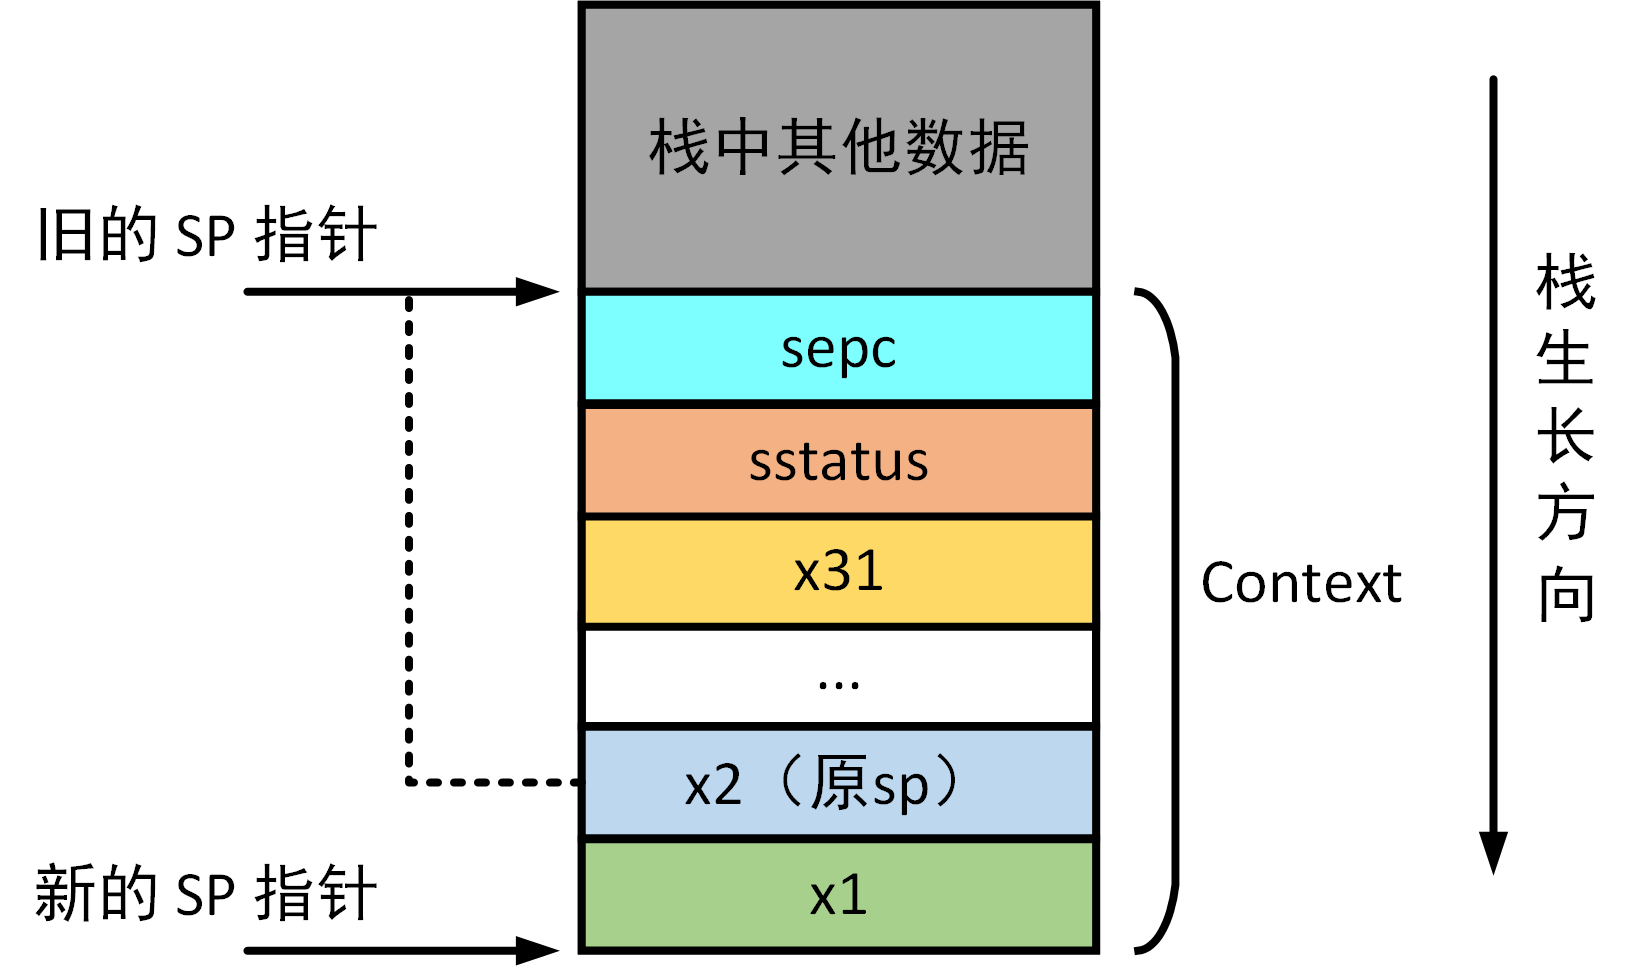
\includegraphics[width=0.55\textwidth]{interruptframe}
	\setlength{\abovecaptionskip}{2pt}
	\caption{保存中断上下文}
	\label{pic:interruptframe}
\end{figure}

完成这些操作后,Moonix就调用了handleInterrupt()函数,并将刚刚保存在内核栈上的InterruptContext地址,以及scause和stval作为参数传入函数。在handleInterrupt()函数中,就会根据scause寄存器的值来确定中断类型,并调用对应的中断处理函数来具体处理。

\subsection{恢复中断上下文}

中断处理结束后,需要从内核栈上恢复上下文,并跳转到原来中断发生时程序执行的位置。

此时sscratch已经在保存上下文时清零了。如果中断发生前CPU处于U-Mode,Moonix需要在返回前将sscratch置为内核栈顶的地址,内核栈顶地址已经保存在寄存器s0中,只需要减去InterruptContext占据的空间即可。

由于此时sscratch已经无法用于判断中断前模式,恢复时借助sstatus寄存器的SPP位。整个恢复过程如代码 \ref{lst:restorecontext} 所示。

Moonix最后执行sret指令,控制流将跳转到sepc寄存器中保存的地址处,即中断发生的位置。同时,CPU会被设置为sstatus中的SPP位标记的模式,由于中断处理过程中没有对sstatus寄存器做过修改,所以会切换会进入中断前的模式。

在Moonix线程创建时,将借助中断恢复的机制来对线程的模式和寄存器等进行设置填充,以进行初始化。更具体的细节见第 \ref{chapter:thread} 章。

\clearpage

\begin{lstlisting}[language={C}, caption={恢复中断上下文}, label={lst:restorecontext}]
__restore:
	# 恢复 CSR
	LOAD    s1, 32
	LOAD    s2, 33
	# 如果从 S-Mode 进入中断, sstatus 的 SPP 位为 1
	# 如果从 U-Mode 进入中断, sstatus 的 SPP 位为 0
	andi    s0, s1, 1 << 8
	bnez    s0, to_kernel
to_user:
	# 释放内核栈空间
	addi    s0, sp, 34 * REG_SIZE
	# 如果从 U-Mode 进入中断
	# 则此时 sscratch 指向用户栈顶
	# 令其指向内核栈顶地址
	csrw    sscratch, s0
to_kernel:
	# 恢复 sstatus 和 sepc
	csrw    sstatus, s1
	csrw    sepc, s2
	# 恢复通用寄存器
	LOAD    x1, 1
	# 恢复 x3 至 x31
	.set    n, 3
	.rept   29
		LOAD_N  %n
		.set    n, n + 1
	.endr
	# 最后恢复 sp(这里最后恢复是为了上面可以正常使用 LOAD 宏)
	LOAD    x2, 2
	sret
\end{lstlisting}

\section{条件变量与标准输入缓冲的实现}
\label{sec:condition}

条件变量在Moonix中,主要用于实现标准输入缓冲。条件变量和标准输入缓冲主要基于这样的场景提出的:一个用户进程通过getc()函数发起了一个系统调用,用于获取一个键盘输入的字符,内核处理调用的时候发现,当前并没有字符输入。这时,一个很简单的想法就是进入一个忙循环,不断地检查是否有字符输入,直到有字符输入后再将其读出,系统调用返回。这种方式肯定能保证读到字符,但是线程会占用资源,什么都不做,浪费CPU资源,即使会被CPU调度,但是所有属于该线程的时间片都被浪费掉了。

Moonix使用条件变量机制来解决这个问题,当线程检查到当前没有键盘输入时,就自动进入睡眠状态,同时不再参与调度,直到有字符输入时,才会将这个线程唤醒参与调度,这个时候被唤醒的线程就一定可以获取到字符并返回了。这样这个问题就被转化成了一个典型的生产者消费者问题。

标准输入缓冲维护了一个字符队列和一个条件变量,而条件变量也只是维护了一个等待队列,保存了等待条件满足的线程的tid。Moonix定义结构如代码 \ref{lst:stdin} 所示。

\begin{figure}[htpb]
\begin{lstlisting}[language={C}, caption={标准输入缓冲和条件变量}, label={lst:stdin}]
typedef struct {
	Queue waitQueue;
} Condvar;

struct
{
	Queue buf;
	Condvar pushed;
} STDIN;
\end{lstlisting}
\end{figure}

当一个线程排队进入临界区尝试获取输入的字符时,如果字符队列中有字符,则直接获取返回。若无字符,则将自身放入等待队列中并挂起。当有字符被输入时,Moonix会首先将字符存入字符队列,并检查等待队列中是否有线程在等待,如果有则唤醒队首线程,该线程会重新尝试进入临界区获取字符。整个流程示意如图 \ref{pic:stdin}。

\begin{figure}[htpb]
	\centering
	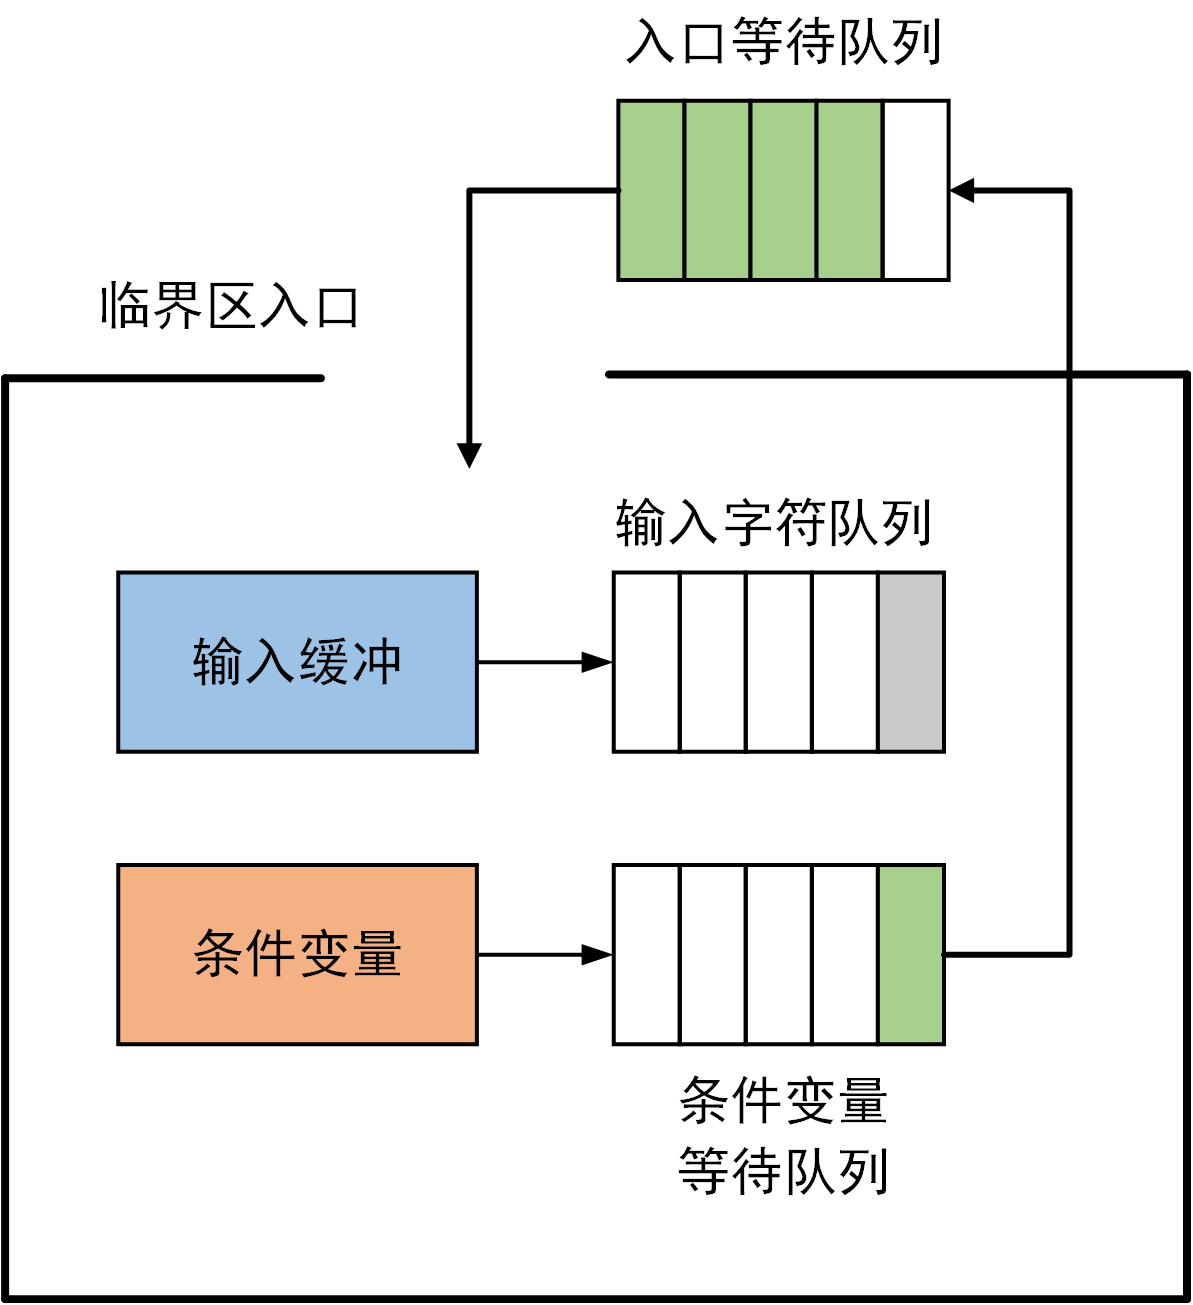
\includegraphics[width=0.4\textwidth]{stdin}
	\setlength{\abovecaptionskip}{2pt}
	\caption{标准输入缓冲区示意}
	\label{pic:stdin}
\end{figure}